\documentclass[a4paper]{article}
\usepackage[utf8]{inputenc}
\usepackage[usenames,dvipsnames]{color}
\usepackage{ngerman}
\usepackage{textcomp}
\usepackage{longtable}
\usepackage{amssymb}
\usepackage{helvet}
\usepackage{graphicx}
\usepackage{setspace}
\usepackage[super,square]{natbib}
\usepackage[colorlinks=true,linkcolor=black,citecolor=black,urlcolor=blue]{hyperref}
\usepackage[rflt]{floatflt}
\usepackage{geometry}
\usepackage{listings}
\usepackage{fancyhdr}
\geometry{a4paper,left=30mm,right=30mm,top=25mm,bottom=25mm}
% \renewcommand{\rmdefault}{\sfdefault}
\renewcommand{\headrulewidth}{0.0pt}

\newcommand{\cfile}[1]{\texttt{#1}}
\newcommand{\ccaption}[1]{\textsc{#1}}
\newcommand{\cvalue}[1]{\texttt{#1}}
\newcommand{\ckeyword}[1]{\texttt{#1}}

\newcommand{\note}[1]{\textbf{Hinweis:} #1 \par}
\newcommand{\warning}[1]{\textbf{Warnung:} #1 \par}

\newcommand{\rarrow}{\textrightarrow}

\onehalfspacing

\lstset{
    basicstyle=\footnotesize\ttfamily, numbers=left, numberstyle=\footnotesize\ttfamily,
    keywordstyle=\color{blue}\bfseries, commentstyle=\color{Gray}\textit, stringstyle=\color{Maroon},
    stepnumber=1, numbersep=10pt, backgroundcolor=\color{white},
    frame=l, tabsize=2, captionpos=b, breaklines=true, breakatwhitespace=true,
    showspaces=false, showtabs=false, showstringspaces=false,
    title=\lstname, escapeinside={\%*}{*)},
    morekeywords={__file__}
}

\begin{document}

\pagestyle{fancy}
\fancyhf{}
\fancyfoot[R]{\huge{\thepage}}

\vspace*{\fill}
\begin{center}
  \Huge{\textbf{ORCF Custom Content Guide}} \\
  \vspace{2cm}
  \large{F"ur ORCF \textbf{2011.09p}} \\
  \vspace{1cm}
  \large{\today}
  \vspace{3cm}
\end{center}
\vfill

\newpage

\tableofcontents

\newpage

\section{Custom Content und ORCF}
ORCF wurde von Anfang an darauf ausgelegt, von den Usern um eigene Objekte erweitert zu werden -- mit allen M"oglichkeiten, die das Spiel bietet. Dazu ist
diese Anleitung gut, auch wenn die garantiert noch nicht fertig ist, aber hey, das Spiel selbst ist ja auch noch alles andere als fertig und das einzige,
was man bisher erstellen kann, sind einfache Objekte zum Hinstellen. Die k"onnen zwar auch animiert sein -- daf"ur muss man aber etwas programmieren. Auf
die Programmierung wird aber erst in einer zuk"unftigen Ver"offentlichung eingegangen, wenn das System etwas ausgereifter ist.

\subsection{Das Standardpaket}
Alle Objekte, die in dieser Vorabversion enthalten sind, fliegen selbstverst"andlich raus. Die wurden nur erstellt um grafische Effekte zu demonstrieren
und um etwas rumzuspielen.

Wenn ihr Lust habt, k"onnt ihr Sets f"ur das so genannte Standardpaket erstellen, damit es standardm"a"sig bei ORCF mitgeliefert wird. Allerdings gibt es
da neben einigen technischen Anforderungen, die sp"ater erw"ahnt werden, einige Voraussetzungen:
\begin{itemize}
\item
  Die Sets m"ussen unter einer Creative Commons-Lizenz stehen, die mindestens die unver"anderte nichtkommerzielle Weitergabe mit Namensnennung erlaubt,
  vorzugsweise auch noch Ver"anderungen am Original, damit das Set nicht von den Erstellern selbst an technische "Anderungen angepasst werden muss. Ein
  Beispiel ist die Lizenz CC BY-NC-SA 3.0.
\item
  Um darauf hinzuweisen, was erlaubt ist, ist dem Set eine \cfile{readme.txt} beizulegen.
\item
  Sie d"urfen demnach keine Inhalte, die nicht unter einer zu der gew"ahlten Creative Commons-Lizenz stehen, enthalten. Das gilt vor Allem f"ur Texturen.
\end{itemize}


\section{Voraussetzungen}

\subsection{Blender}
Das mitgelieferte Export-Script f"ur Objekte funktioniert nur mit Blender 2.5. Ihr ben"otigt also eine aktuelle Version von Blender sowie grundlegende
Kenntnisse im Umgang mit der Software. Wenn ihr mit Blender 2.4 arbeitet, werdet ihr in 2.5 wahrscheinlich nicht sofort alles an gewohnter Stelle
finden.

\subsection{Das Export-Script}
Im Unterordner \cfile{tools} befindet sich neben zwei ausf"uhrbaren Programmen die Datei \cfile{export.py}. Bevor ihr diese zu Blender hinzuf"ugt,
m"usst ihr allerdings die Pfade zu einigen ORCF-eigenen Hilfsprogrammen angeben. Wenn ihr die Datei in einem Texteditor "offnet, der Zeilenumbr"uche
unterst"utzt (z.\, B. Kate, Notepad++, \dots ), findet ihr recht weit oben folgende Zeilen:
\begin{lstlisting}[language=python]
ocfgen_exe = '...'
orcf_data_path = '...'
orcf_personal_data_path = '...'
\end{lstlisting}

\subsubsection{Windows}
Unter Windows sieht das beispielsweise so aus:
\begin{lstlisting}[language=python]
ocfgen_exe = 'C:/orcf/tools/ocfgen.exe'
orcf_data_path = 'C:/orcf/data/'
orcf_personal_data_path = 'C:/orcf/data/'
\end{lstlisting}

Beachtet bitte, dass Python auch unter Windows einfache Schr"agstriche bei Pfaden akzeptiert und dass die letzten beiden Pfade identisch sein m"ussen!

\subsubsection{Linux}
Unter Linux liegt der letzte Pfad immer im Userverzeichnis und hei"st immer \cfile{orcf-data}. Die
anderen beiden Pfade zeigen dahin, wo das Programm liegt -- vorzugsweise in \cfile{/opt/orcf}, wenn es f"ur alle Systembenutzer zug"anglich sein soll.


\section{Ordnerstruktur eines Sets}
\label{directories}
Objekte liegen \emph{immer} im \cfile{scenery}-Ordner in einem der Datenordner -- es ist dabei v"ollig egal, ob es der pers"onliche Datenordner oder der
Systemordner ist. In der ersten Ebene liegen dabei die OCF-Dateien, die auf die einzelnen Objekte im Set
verweisen, sowie die Ordner, in denen die eigentlichen Daten eurer Sets liegen. Damit es nicht zu "Uberschneidungen kommt, benennt eure Ordner und
OCF-Dateien m"oglichst nach folgendem Schema:\\
\cfile{Name\_des\_Erstellers-Name\_des\_Sets} f"ur den Ordner und \\
\cfile{Name\_des\_Erstellers-Name\_des\_Sets.ocf} f"ur die OCF-Datei.

Innerhalb des Ordners seid ihr theoretisch v"ollig frei in der Namensgebung. Es sollten jedoch nur "`normale"' Zeichen verwendet werden, d.\,h.
Buchstaben, Zahlen sowie Unter- und Bindestriche. Leerzeichen f"uhren jedoch zu Problemen.

Weil das Export-Script eine Menge Dateien erzeugt, die durchaus bei verschiedenen Objekten denselben Namen haben k"onnen, ist es empfehlenswert, f"ur
jedes Objekt einen eigenen Ordner anzulegen.

\section{Objekte erstellen}
Voraussetzung ist, dass ihr mit Blender modellieren und texturieren k"onnt. Hier sollen nur die Spezialit"aten von Blender im Bezug auf ORCF-Objekte
erl"autert werden, nicht aber die Grundlagen, denn das w"urde zu viel Zeit in Anspruch nehmen -- es gibt mehr als genug gute Blender-Tutorials da
drau"sen.

\subsection{Informationen "uber das Objekt}
Die meisten Angaben hierzu werden in ORCF selbst angegeben -- der Name des Autors steht allerdings in der Blender-Datei. Um diesen zu setzen, erstellt ihr
im World-Panel ein Custom Property mit dem Namen \ccaption{author} und eurem Namen als Wert:
\begin{center}
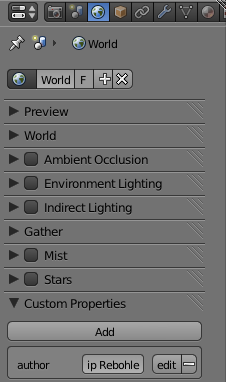
\includegraphics[width=40mm]{../images/blender/world-author.png}
\end{center}
Diese Information wird bei jeder Datei ben"otigt, also kann es sich durchaus lohnen, ein Template zu erstellen, in dem das bereits drinsteht.

\subsection{Materialien}
Vorweg: Gebt euren Materialien aussagekr"aftige Namen! Jedes einzelne Material kann im Spiel vom Nutzer ver"andert werden (v.\,a. die Farbe), da hilft
es wenig, wenn das Material "`Material.005"' hei"st. Leerzeichen sorgen aber f"ur Probleme bei der OCF-Dateierstellung, verwendet also statt Leerzeichen
bitte Unterstriche. Umlaute sind auch verboten, weil Windows Umlaute anders codiert als andere Systeme -- hier gilt also dasselbe wie schon bei der
Benennung der Dateien weiter oben.

\warning{Nutzt Transparenz bitte nur, wenn n"otig (z.\,B. bei Fenstern), denn das Rendering von transparenten Objekten ist in ORCF schlecht implementiert
  und f"uhrt zu Anzeigeproblemen.}

\subsubsection{Benutzbare Eigenschaften}
\begin{itemize}
\item Materialfarbe (\ccaption{Diffuse}, \ccaption{Diffuse \rarrow Intensity}). Kann vom Spieler ge"andert werden.
\item Emission (\ccaption{Shading \rarrow Emit}). Aktiv f"ur selbstleuchtende Materialien. Kann vom Spieler ge"andert werden.
\item Glanzlicht-Intensit"at (\ccaption{Specular \rarrow Intensity})
\item Glanzlicht-H"arte (\ccaption{Specular \rarrow Hardness})
\item Durchsichtigkeit (\ccaption{Transparency \rarrow Alpha})
\item Reflexionsst"arke (\ccaption{Mirror \rarrow Reflectivity})
\item Reflexionsmodus (\ccaption{Mirror \rarrow Max Distance}). Ein Wert von \cvalue{0} bedeutet, dass \emph{immer} eine fast statische Environment Map
  auf das Objekt gelegt wird (empfehlenswert bei Objekten mit geringer Reflexionsst"arke sowie sehr gro"sen Objekten), jeder gr"o"sere Wert bedeutet, dass
  die Reflexionstextur dynamisch gerendert wird, wenn der User dies in den Grafikeinstellungen aktiviert hat
\item Texturen, dazu aber mehr im Abschnitt \ref{objects_textures} Texturen.
\end{itemize}

\subsubsection{Custom Properties}
\begin{itemize}
\item \ccaption{displacementHeight} -- betrifft nur User mit aktiviertem Parallax Occlusion Mapping. Gibt die maximal simulierte Tiefe in Metern an,
      Standardwert ist \cvalue{0.04}, Werte bis \cvalue{0.20} erzeugen in der Regel gute Ergebnisse.
\end{itemize}

\subsection{Texturen}
\label{objects_textures}
ORCF kann zwei verschiedene Typen von Texturen verarbeiten: Farbtexturen und Bump Maps. Bump Maps sind Texturen, die Informationen "uber die Ausrichtung
und die Verschiebung von der Oberfl"ache eines Objekts enthalten, um den Detailgrad ohne zus"atzliche Polygone deutlich zu erh"ohen. Die Erstellung von
Bump Maps mit Blender wird im Abschitt \ref{bumpmaps} Bumpmaps erl"autert.
\note{Bitte sorgt daf"ur, dass eure Farbtexturen nur dann einen Alphakanal haben, wenn er wirklich genutzt wird! Sonst funktionieren Dinge wie Parallax
  Occlusion Mapping nicht und es kommt zu unsch"onen Artefakten.

\subsubsection{Benutzbare Eigenschaften}
\begin{itemize}
\item Typ muss \cvalue{Image or Movie} sein
\item \ccaption{Image \rarrow Source} muss auf eine TGA-Datei verweisen
\item \ccaption{Mapping \rarrow Coordinates} muss auf \cvalue{UV} stehen
\item bei \ccaption{Influence} kann entweder \cvalue{Color} oder \cvalue{Normal} aktiviert werden. Wenn \cvalue{Color} aktiv ist, so wird die Farbe
  der Textur im Spiel mit der gew"ahlten Materialfarbe multipliziert -- wenn euer Objekt also einf"arbbar sein soll, achtet darauf, dass eure Textur
  m"oglichst nur Graut"one beinhaltet. Wenn \cvalue{Normal} aktiv ist, handelt es sich um eine Bumpmap.
\end{itemize}

\subsection{Objekte}
Das, was in ORCF als Mesh bezeichnet wird, hei"st in Blender "`Object"' und stellt die Geometrie dar.

\subsubsection{Benutzbare Eigenschaften}
\begin{itemize}
\item Position (\ccaption{Transform \rarrow Location}). Ergibt sich, wenn man im Object Mode das Objekt verschiebt.
\item Drehung (\ccaption{Transform \rarrow Rotation}). Ergibt sich, wenn man im Object Mode das Objekt dreht.
\item Elternobjekt (\ccaption(Relation \rarrow Parent}). Alle Transformationsoperationen des Elternobjekts werden auch auf dieses Objekt "ubertragen,
  besonders bei Animationen interessannt.
\end{itemize}
\warning{Die Skalierung (\ccaption{Transform \rarrow Scale}) kann \emph{nicht} benutzt werden! Wenn ihr skaliert, tut dies \emph{immer} im Edit Mode.}

\subsubsection{Custom Properties}
\begin{itemize}
\item \ccaption{min\_dist} -- falls mehrere LODs benutzt werden, gibt dies die minimale Distanz an, die das Objekt zum Betrachter haben muss, um an-
  gezeigt zu werden. Wenn keine LODs benutzt werden oder das Objekt den h"ochstm"oglichen Detailgrad besitzt, sollte diese Eigenschaft nicht benutzt
  werden.
\item \ccaption{max\_dist} -- falls mehrere LODs benutzt werden, gibt dies die maximale Distanz an, die das Objekt zum Betrachter haben muss, um an-
  gezeigt zu werden. Wenn keine LODs benutzt werden oder das Objekt den niedrigsten Detailgrad besitzt, sollte diese Eigenschaft nicht benutzt
  werden.
\end{itemize}

\subsection{Lampen}
Vorweg: Um eine Lampe in ORCF verwenden zu k"onnen, muss sie als Parent ein Objekt haben. Au"serdem hat ORCF ein "ahnliches Beleuchtungsmodell wie
Blender, die genauen Berechnungen sind aber doch anders, deswegen sehen die Ergebnisse beim Rendern nicht zwangsl"aufig gleich aus.

\subsubsection{Benutzbare Eigenschaften}
\begin{itemize}
\item Position -- ergibt sich, wenn die Lampe verschoben wird.
\item Typ muss \cvalue{Point} sein
\item Schatten (\ccaption{Shadow}) muss auf \cvalue{Ray Shadow} gesetzt werden, wenn die Lampe Schatten werfen soll.
\item Farbe (\ccaption{Lamp}) -- wird in zuk"unftigen ORCF-Versionen auch vom Spieler ge"andert werden k"onnen. Erstellt daher bitte nicht f"ur
  verschiedene Beleuchtungsfarben eigene Objekte.
\item Energie (\ccaption{Lamp \rarrow Energy}) -- wird ebenfalls eines Tages vom Spieler ge"andert werden k"onnen.
\item Leuchtweite (\ccaption{Lamp \rarrow Energy}) -- gibt an, in welcher Entfernung die Lampe nur noch die H"alfte ihrer urspr"unglichen Leuchtkraft
  besitzt. Wird ebenfalls eines Tages vom Spieler ge"andert werden k"onnen.
\end{itemize}

\subsubsection{Custom Properties}
\begin{itemize}
\item \ccaption{onlyNight} -- der Wert spielt hier keine Rolle, wenn die Eigenschaft gesetzt ist, leuchtet die Lampe nur bei Nacht.
\end{itemize}

\subsection{Ein paar Dinge\dots }
ORCF ist nicht RCT3. Es beherrscht gerade in Sachen Platzierung viele Dinge, die RCT3 nicht kann. Daher solltet ihr folgendes beachten:
\begin{itemize}
\item Nutzt die M"oglichkeit von Parallax Occlusion Mapping aus. Das spart oft sehr viele Polygone und kann den Detailgrad extrem erh"ohen.
\item Wenn ihr Alphamasken nutzt, um detailreiche Objekte mit einem einzelnen Polygon zu rendern, beachtet bitte, dass hier kein Parallax Occlusion
  Mapping funktioniert und dass an den R"andern der Textur (noch) Artefakte auftreten k"onnen.
\item Objekte lassen sich beliebig drehen und spiegeln. Ihr braucht also f"ur Seitenr"ander von D"achern nicht 2 Objekte erstellen, eines reicht.
\item Bumpmaps und Farbtexturen benutzen dieselben Texturkoordinaten!
\item In zuk"unftigen Versionen werden einfache Objekte wie W"ande skalierbar sein, sodass der Eindruck entsteht, es st"unden mehrere W"ande
  nebeneinander. Die meisten W"ande sollten deshalb nur ein Mal mit einer Gr"o"se von 2x2x0.2 Metern abgespeihert werden. \note{Das gilt jedoch
  nicht f"ur W"ande, die sich nicht kacheln lassen -- wenn also zum Beispiel eine Wand mit Basis erstellt wird, so w"urde eine Skalierung in die H"ohe
  das Problem mit sich bringen, dass die Basis nicht nur direkt "uber dem Boden sichtbar ist. Hier ist es n"otig, eine Wand ohne Basis zu erstellen,
  die sich dann wieder kacheln l"asst.}
\item Verschiebt die Objekte so in der H"ohe, dass die Stellen, die den Boden ber"uhren sollen, auf dem Koordinatensystem von Blender die H"ohe 0 haben.
  So lassen sich Objekte einfacher platzieren und stapeln.
\item ORCF wird in zuk"unftigen Versionen die M"oglichkeit erhalten, Objekte wie Z"aune an schr"age Stellen wie bspw. einen Terrainh"ugel oder einer
  Bogenbr"ucke auszurichten. Ihr braucht demnach keine Objekte erstellen, in denen diese Abschr"agung bereits vorhanden ist.
\item Benutzt LODs, wo es sinnvoll ist -- aber bitte nicht zu viele. Drei Detailstufen sind in der Regel vollkommen ausreichend.
\item Einfarbige Fl"achen ben"otigen keine Textur.
\end{itemize}

\subsection{Linken von externen Ressourcen}
Ihr k"onnt, um eine Menge Ressourcen zu sparen, Materialien und vor Allem Texturen aus vorher erstellten Blender-Dateien einbinden. Dazu geht ihr
im \ccaption{File}-Men"u auf \ccaption{Link}, w"ahlt die Datei aus und sucht dort das entsprechende Material oder die entsprechende Textur. Diese lassen
sich dann auf herk"ommliche Weise ausw"ahlen, als w"aren sie in die Datei integriert.

Das sorgt daf"ur, dass die gelinkten Daten nicht mit in die OCF-Datei geschrieben werden und auch im Spiel nicht mehrfach geladen werden. Das spart
Speicherplatz auf der Festplatte und auf der Grafikkarte, und gerade da sollte man sehr sparsam sein. Diese Funktionalit"at entspricht etwa
den aus RCT3 bekannten Shared Textures. Nicht m"oglich ist das allerdings bei Objekten, die Geometrie muss also jedes mal mit exportiert werden.

\section{Bumpmaps erstellen mit Blender}
\label{bumpmaps}
Hier soll kurz erkl"art werden, wie man mit Blender eine Bumpmap aus einem Objekt erstellt.

\subsection{Das Objekt}
Das Objekt wird nicht ins Spiel importiert. Es dient lediglich dazu, Polygone in den eigentlichen Objekten einzusparen, ohne jedoch an Detailreichtum
einzub"u"sen -- daher muss hier bei diesem Objekt keine R"ucksicht auf die Anzahl der Polygone genommen werden. Im Grunde erstellt ihr hier genau das, was
ihr ansonsten in das Objekt mit eingebaut h"attet, beispielsweise Dachziegel.

\subsection{Das Material}
Ihr weist dem Objekt allerdings nicht die Farben zu, die das Objekt, das die Bumpmap nutzt, sp"ater haben soll. Der Trick liegt darin, das Objekt ohne
Farben und ohne Beleuchtung zu rendern. Dazu f"arbt ihr das Material schwarz und aktiviert \ccaption{Shading \rarrow Shadeless}, au"serdem muss f"ur die
H"oheninformationen noch \ccaption{Transparency} aktiviert und der Modus auf \cvalue{Mask} gestellt werden.
\begin{center}
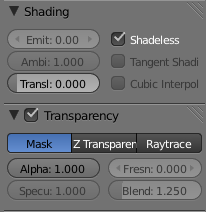
\includegraphics[width=40mm]{../images/blender/bumpmap-material.png}
\end{center}

\subsection{Die Normalentexturen}
Hier liegt eigentlich das Geheimnis. Blender kann mit einigen Tricks die Normale als Farbinformationen auf das Material legen. Dazu m"usst ihr verstehen,
wie eine Bumpmap eigentlich aussieht:

Jeder Pixel auf der Bumpmap repr"asentiert einen Normalenvektor aus den Komponenten X, Y und Z. Die Werte liegen dabei alle zwischen -1 bis 1 -- auf der
Textur werden sie durch rote, gr"une und blaue Farbkomponenten mit einem Wertebereich von 0 bis 255 dargestellt. Zun"achst erstellt ihr also eine Textur
f"ur die Z-Komponente der Normale. Die ist blau und muss genau dieselben Eigenschaften haben wie unten dargestellt:

\begin{center}
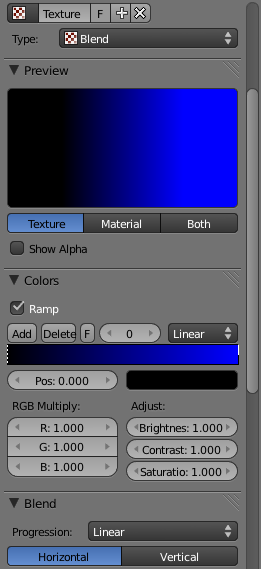
\includegraphics[width=40mm]{../images/blender/bumpmap-texture-1.png}
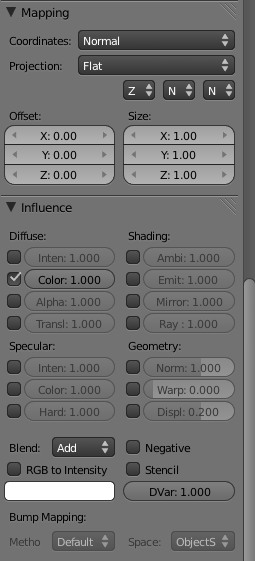
\includegraphics[width=40mm]{../images/blender/bumpmap-texture-2.png}
\end{center}

Wichtig ist, dass das Blau ein reines und volles Blau ist, also keine anderen Farbanteile mehr vorhanden sind.

Am Wichtigsten ist hier die Einstellung \ccaption{Mapping \rarrow Coordinates}. Mit dem Wert \cvalue{Normal} wird Blender angewiesen, die Normalen als
Quelle f"ur das Texturmapping zu verwenden.

Unter \ccaption{Mapping \rarrow Projection} finden sich 3 Auswahlboxen. Die erste davon steht auf \cvalue{Z}, die anderen beiden auf \cvalue{N}. Damit
teilen wir der Blender mit, dass nur der Z-Anteil der Normale ber"ucksichtigt werden soll.

Achtet aber auch darauf, bei \ccaption{Influence \rarrow Blend} \cvalue{Add} auszuw"ahlen, denn sonst seht ihr immer nur eine der drei Texturen.

Ihr m"usst jetzt noch zwei weitere Texturen erstellen, eine rote f"ur die X-Anteile und eine gr"une f"ur die Y-Anteile. Dazu muss lediglich die Farbe
ge"andert werden und das Mapping ist von \cvalue{Z} auf \cvalue{X} bzw. \cvalue{Y} zu stellen.

Am Ende sollte die Materialvorschau etwa folgendes ausspucken:

\begin{center}
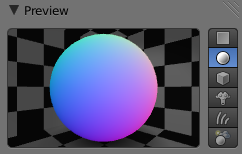
\includegraphics[width=40mm]{../images/blender/bumpmap-material-preview.png}
\end{center}

\subsection{Die H"ohentextur}
Damit Parallax Occlusion Mapping mit dieser Bumpmap funktioniert, m"usst ihr noch eine Alphatextur erstellen. Die ist sehr "ahnlich zu den
Normalentexturen, allerdings mit den folgenden Unterschieden:
\begin{itemize}
\item Die Textur geht nicht von Schwarz zu einer Farbe, sondern von voll durchsichtig zu wei"s.
\item Das Mapping benutzt nicht die Z-Komponente der Normale, sondern die Z-Position im World Space (dazu die Einstellung \cvalue{Global} bei
  \ccaption{Mapping \rarrow Coordinates}.
\end{itemize}

Alles in Allem sollte das etwa so aussehen:

\begin{center}
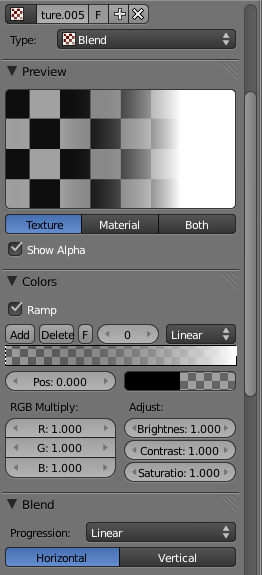
\includegraphics[width=40mm]{../images/blender/bumpmap-texture-3.png}
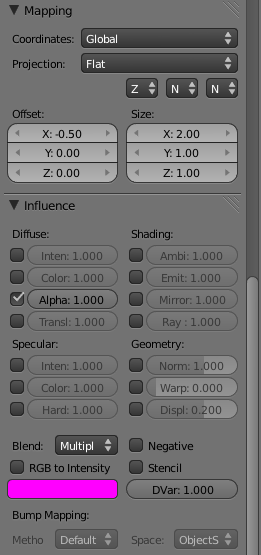
\includegraphics[width=40mm]{../images/blender/bumpmap-texture-4.png}
\end{center}

Offset und Size sind dabei so gew"ahlt, dass f"ur ein Objekt, dessen Z-Werte zwischen 0 und 1 liegen, eine perfekte Alpha-Map erstellt wird. F"ur andere
Wertebereiche m"usst ihr gegebenenfalls etwas rumexperimentieren, oft ist es aber am einfachsten, das Objekt an die richtige Stelle in der Welt zu
verschieben und zu skalieren. Skaliert euer Objekt aber keinesfalls ausschlie"slich in Z-Richtung, denn dadurch w"urden die Normalen verf"alscht!

\subsection{Die Kamera}
Erstellt eine neue Kamera und setzt diese "uber das Objekt. Wie hoch sie liegt, ist egal, da sie nicht perspektivisch ist, sondern orthogonal. Das sollte
dann etwa so aussehen:

\begin{center}
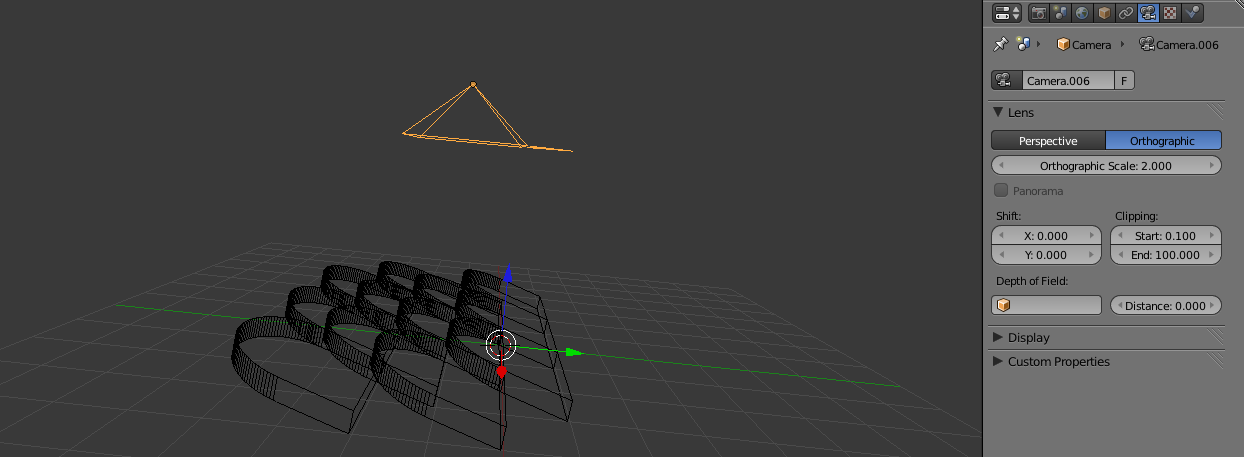
\includegraphics[width=150mm]{../images/blender/bumpmap-camera.png}
\end{center}

Im Scene-Panel k"onnt ihr die neue Kamera dann als Standardkamera festlegen, das ist unter Anderem f"ur Rendervorg"ange n"otig.

Wie ihr \ccaption{Orthographic Scale} w"ahlt, h"angt letztenendes von euerm Objekt ab. Von der Kamera aus sollte das gesamte Objekt sichtbar sein,
ggf. ist es aber n"otig, dass nur ein Teil sichtbar ist, damit die Textur kachelbar bleibt, wie hier im Beispiel mit den Dachziegeln.

\subsection{Rendereinstellungen}
Damit die Bumpmap auch unverf"alscht auf den Bildschirm gebracht wird, m"usst ihr zun"achst Blenders Farbkorrekturen abstellen und RGBA-Rendering
aktivieren. Das geht mit den folgenden Einstellungen im Render-Panel:

\begin{center}
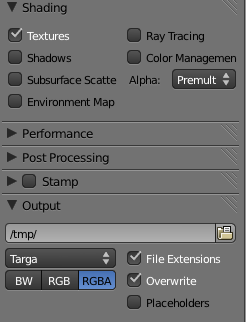
\includegraphics[width=40mm]{../images/blender/bumpmap-render.png}
\end{center}

W"ahlt au"serdem eine passende Gr"o"se, oftmals sind Bumpmaps von 256x256 Pixeln Gr"o"se v"ollig ausreichend.

\subsection{Und.. Rendern!}
Nun sind alle Einstellungen getan und ihr k"onnt die Bumpmap rendern. Bei den Dachziegeln sieht diese etwa so aus, wenn man in Blenders Bildansicht
die Alphakanaldarstellung aktiviert:

\begin{center}
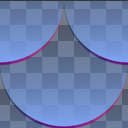
\includegraphics[width=40mm]{../images/blender/bumpmap.png}
\end{center}

Das Bild muss nun noch gespeichert werden. Dazu w"ahlt ihr im \ccaption{Image}-Men"u den Eintrag \ccaption{Save as Image} aus. Wichtig ist dabei,
dass als Dateiformat \cvalue{Targa} ausgew"ahlt ist.
\begin{center}
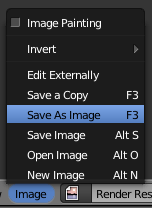
\includegraphics[width=30mm]{../images/blender/image-menu.png}
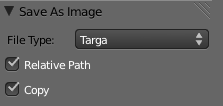
\includegraphics[width=40mm]{../images/blender/blender-image-saving.png}
\end{center}

Und das Ganze dann im Spiel auf zwei Dreiecke gemappt:
\begin{center}
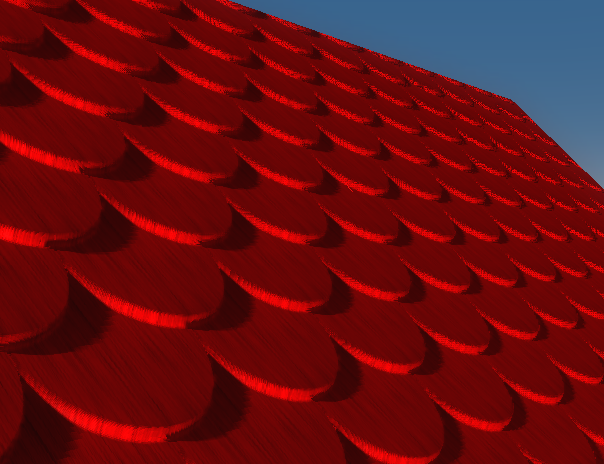
\includegraphics[width=40mm]{../images/blender/bumpmap-ingame.png}
\end{center}

\section{Exportieren}
Im Normalfall gen"ugt ein Klick auf den entsprechenden Men"ueintrag:

\begin{center}
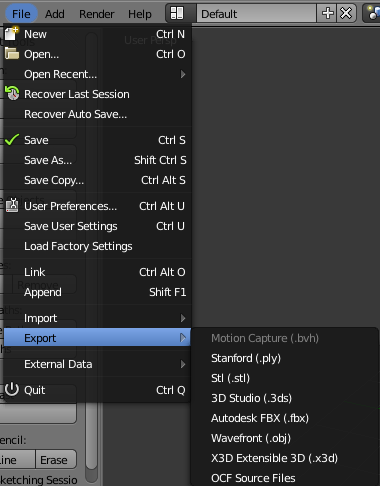
\includegraphics[width=60mm]{../images/blender/blender-menu.png}
\end{center}

Solltet ihr eine Fehlermeldung erhalten, probiert folgendes:
\begin{itemize}
\item Speichert die Datei und ladet sie einmal neu. Das sorgt daf"ur, dass unbenutzte Datenbl"ocke wirklich gel"oscht werden, und somit den Exporter nicht
  weiter st"oren.
\item Wenn das nichts hilft, "offnet in Blender eine Pythonkonsole und gebt folgendes ein:
  \begin{lstlisting}[language=python]
  bpy.ops.export_scene.ocf("/da/wo/eure/Blenderdatei/liegt/")
  \end{lstlisting}
  und schaut auf die Ausgabe. Die Meldung kann auf fehlerhafte Eingaben zur"uckzuf"uhren sein, aber auch auf einen Bug im Script.
\item Sollte das Script durchlaufen, aber keine OCF-Datei in dem Ordner, wo auch eure Blenderdatei ist, auftauchen, so liegt das Problem bei der finalen
  Erstellung der OCF-Datei aus den Einzeldateien. "Offnet eine Kommandozeile in dem Ordner, in dem eure Blender-Datei liegt und f"uhrt die
  \cfile{.bat}-Datei (Windows) bzw. die \cfile{.sh}-Datei (Linux, Mac OS X) aus, die sich in dem Ordner befindet. Fehler dieser Art sind oft auf
  fehlerhafte Benennungen von jeglichen Objekten in Blender zur"uckzuf"uhren, besonders Leerzeichen und Umlaute sorgen hier f"ur Probleme, aber es kann
  genau so gut auch an einem Bug liegen.
\end{itemize}

\section{Vorschaubilder}
Damit der Spieler sofort in der Objektliste des Spiels sieht, wie welches Objekt aussieht, solltet ihr sinnvolle Vorschaubilder erstellen. Das geht auch
direkt in Blender.

\subsection{Allgemeines}
Es sollte auf dem Bild nur das Objekt zu sehen sein, und zwar so gro"s wie m"oglich. Wenn das Objekt nur mit einem anderen Objekt sinnvoll benutzt werden
kann, so ist es ideal, wenn gezeigt wird, wie man das Objekt genau benutzt, indem zum Beispiel das zus"atzlich ben"otigte Objekt ebenfalls integriert.

\subsection{Rendereinstellungen}
Die Gr"o"se eines Vorschaubilds in ORCF betr"agt exakt 96x96 Pixel. Zwar funktioniert die Vorschau auch mit anderen Gr"o"sen, allerdings sieht alles,
was kleiner ist, ziemlich h"asslich aus, und alles, was gr"o"ser ist, ist Ressourcenverschwendung. Deswegen solltet ihr euch daran halten. Au"serdem
sollte die Vorschau einen transparenten Hintergrund haben, daher m"usst ihr das RGBA-Rendering aktivieren. Gute Rendereinstellungen f"ur ein Vorschaubild
sehen beispielsweise so aus:
\begin{center}
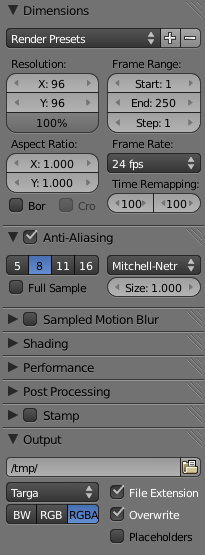
\includegraphics[width=40mm]{../images/blender/preview-rendersettings.png}
\end{center}

Ein Beispielbild eines nicht wirklich sehr gelungenen Holzbodens kann dann zum Beispiel so aussehen:
\begin{center}
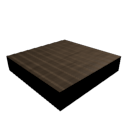
\includegraphics[width=20mm]{../images/blender/preview.png}
\end{center}

\section{Der Set Creator}
\label{setcreator}
Damit eure Objekte auch im Spiel verwendet werden k"onnen, m"usst ihr eine Set-Datei erstellen, die die Objekte referenziert. Erw"ahnt wurde diese
bereits im Abschnitt \ref{directories} Ordnerstruktur eines Sets. Dazu gibt es in ORCF einen so genannten Set Creator, der allerdings etwas versteckt
ist: Klickt im Hauptmen"u auf einen leeren Bereich des Fensters und dr"uckt die Taste \ccaption{s}. Der Set Creator sollte sich "offnen.

\warning{Der Set Creator ist bislang schlecht programmiert. Wenn ihr irgendwo vergesst, einen Namen, eine Beschreibung, eine Kategorie oder ein
Vorschaubild auszuw"ahlen, entsteht ein fehlerhaftes Set, das ihr weder benutzen noch nachtr"aglich ver"andern k"onnt!}

\subsection{Vorschaubilder laden}
W"ahlt den Reiter \ccaption{Previews} aus. Die Oberfl"ache davon d"urfte recht selbsterkl"arend sein: Mit dem gr"unen Plus k"onnt ihr TGA-Bilder laden
und mit dem roten Minus ein ausgew"ahltes Bild wieder entfernen.

\begin{center}
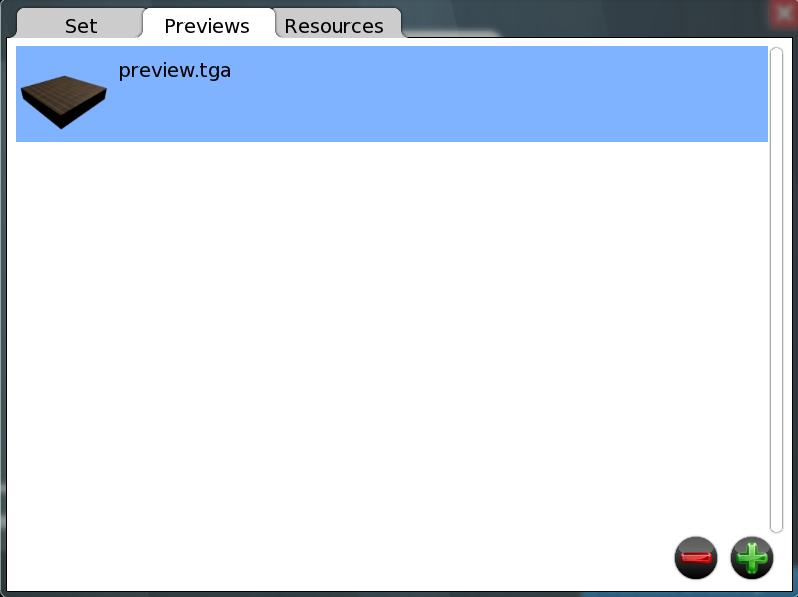
\includegraphics[width=80mm]{../images/setcreator/previews.png}
\end{center}

\subsection{Objekte laden}
Klickt auf den Reiter \ccaption{Resources}. Hier legt ihr fest, welche Objekte im Set vorhanden sind, wie sie hei"sen, wozu sie gut sind und in welchen
Kategorien ("`Tags"') sie erscheinen sollen.

\begin{center}
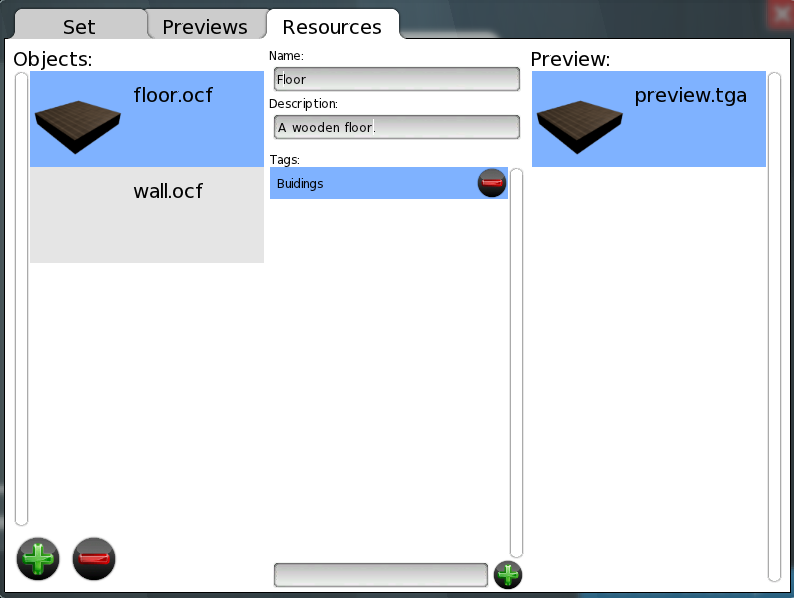
\includegraphics[width=80mm]{../images/setcreator/resources.png}
\end{center}

Die linke Liste enth"alt die Objekte. Mit dem gr"unen Plus k"onnt ihr OCF-Dateien hinzuf"ugen, mit dem roten Minus wieder entfernen. Jedes Objekt hat
einen Namen, eine Beschreibung, eine Liste von Kategorien und ein Vorschaubild. Die geladenen Vorschaubilder werden rechts angezeigt. Um eine dieser
Eigenschaften f"ur ein Objekt zu "andern, m"usst ihr zun"achst in der linken Liste das entsprechende Objekt ausw"ahlen.

\subsubsection{Die Kategorien}
Um auch bei einer gro"sen Anzahl von Objekten die "Ubersicht zu wahren, kann der Nutzer verschiedene Kategorien anw"ahlen. Diese sind allerdings nicht
vom Spiel festgelegt, sondern von den Erstellern des Sets. Da es aber wenig hilft, wenn einer seine Teile in "`D"acher"' einordnet und der n"achste in
"`Dach"', solltet ihr gewisse Regeln beachten.

\begin{itemize}
\item Nutzt englische Begriffe. Nicht jeder spricht Deutsch.
\item Nutzt bei Typenbeschreibungen die Mehrzahl, also "`Walls"' statt "`Wall"'.
\item Orientiert euch an existierenden Kategorien. Wenn schon Objekte in eine Kategorie "`East Asia"' eingeordnet wurden, nutzt diese f"ur entsprechende
  Objekte, anstatt eine neue Kategorie "`China"' o.\,"a. einzurichten. Das wahrt die "Ubersicht.
\item Gebt Kategorien f"ur Themengebiete aussagekr"aftige Namen -- ein Set mit nordischen Elementen macht sich besser in "`Vikings"' als in "`History"'.
\item Nutzt mehrere Kategorien. Ein Atlantis-Dach sollte sowohl in "`Atlantis"' als auch in "`Buildings"' und "`Roofs"' erscheinen.
\end{itemize}

Im Folgenden mal eine Liste von Kategoriennamen, die eingehalten werden sollten:
\begin{itemize}
\item \ccaption{Buildings} -- Alles, was mit Geb"auden zu tun hat. D"acher, W"ande usw.
\item \ccaption{Walls} -- Alle m"oglichen W"ande. Also auch Fenster, abgeschr"agte W"ande f"ur D"acher, Ecken usw.
\item \ccaption{Roofs} -- D"acher.
\item \ccaption{Plants \& Trees} -- Pflanzen und B"aume.
\item \ccaption{Fences} -- Z"aune.
\item \ccaption{Lamps} -- Objekte mit Lampen.
\item \ccaption{Particles} -- F"ur Objekte mit Partikeleffekten wie Feuer, Wasser, Staub, Nebel usw. (Noch nicht m"oglich)
\item \ccaption{Sounds} -- F"ur Objekte, die einen Sound abspielen. (Noch nicht m"oglich)
\item \ccaption{Flatrides} -- F"ur Flatrides. (Noch nicht m"oglich)
\item \ccaption{Tracked Rides} -- Achterbahnen, Wasserbahnen etc. (Noch nicht m"oglich)
\item \ccaption{Stalls} -- L"aden und St"ande. (Noch nicht m"oglich)
\end{itemize}

Ihr k"onnt neue Kategorien in die Liste hinzuf"ugen, indem ihr den Namen der Kategorie in das Textfeld unten eintragt und auf das gr"une Plus klickt.
Die Kategorien, zu denen ein Objekt geh"ort, m"ussen einzeln ausgew"ahlt werden und erscheinen in der Liste mit einem blauen Hintergrund.

\subsection{Informationen zum Set}
Im linken Reiter \ccaption{Set} m"usst ihr zu guter Letzt dem Set einen Namen geben. Verzichtet dabei bitte auf den Namen der Ersteller, diese werden
schon in der Objektliste angezeigt.
\begin{center}
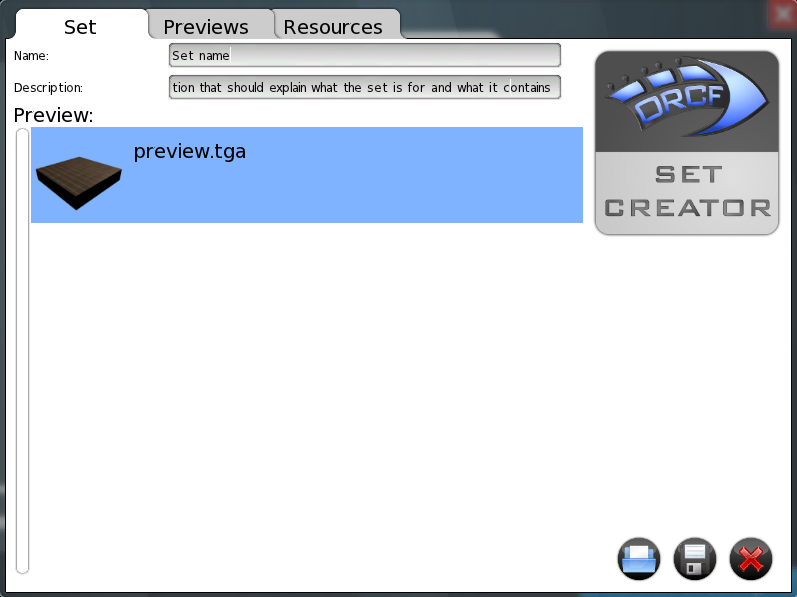
\includegraphics[width=80mm]{../images/setcreator/set.png}
\end{center}

Nun k"onnt ihr das Set abspeichern:
\begin{center}
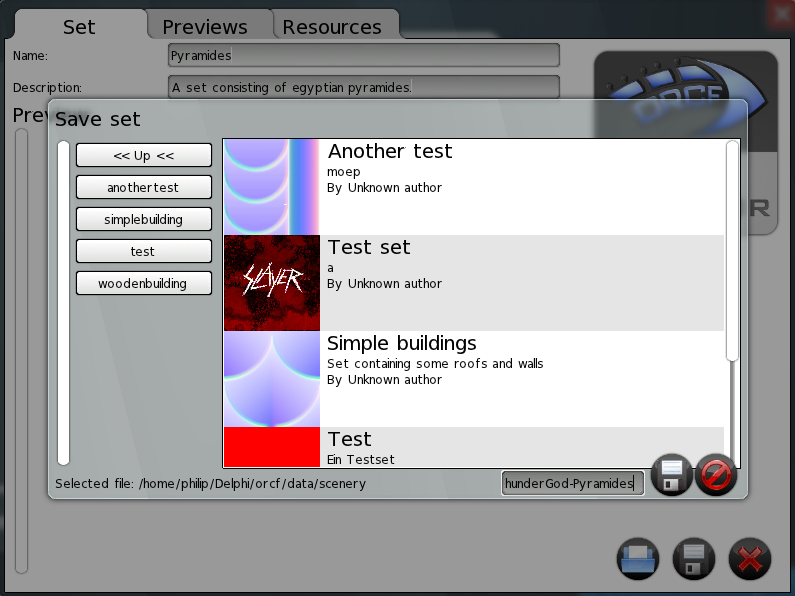
\includegraphics[width=80mm]{../images/setcreator/saving.png}
\end{center}

Beachtet dabei bitte das genannte Dateinamensschema. Der Name sollte dem des Set-Ordners gleichen, die Dateiendung wird automatisch angeh"angt.

\end{document}